\chapter{Introduction}
\label{chap:introduction}


Modeling languages have long played an important role in software engineering. Well designed models can abstract complex systems and provide visual aid in understanding them. Furthermore in form of the Business Process Model Notation (BPMN) they are used to define and automate processes. Today, with research in the area of Model Driven Engineering (MDE), a paradigm centered around models, with the intent to generate code bases and whole systems from them, the importance of models is rising even more.

As these tasks require syntactic correctness of used models, modeling tools become an essential part of an engineer's workflow. Especially visual modeling tools provide in theory, an intuitive and user friendly way to design models. But current graphical modeling tools tend to constraint users in unintuitive ways and deliver sub par user experience (UX). this usually arises from a tight coupling between a modeling tools user interface (UI) and the underlying model. As the model's syntax is usually inflexible, the UI has to make restrictions to adhere to this syntax. this often creates problems for the user, for example connections can only be drawn between two existing states, or deleting a node will result in all its children being deleted as well.

To amend these usability woes, L. Nachreiner proposed a novel modeling framework, called CouchEdit \cite{nachreiner_couchedit_2020}. This framework decouples user interface and model syntax by introducing different models for both. Instead of relying directly on the syntax of the model that is being designed, in the CouchEdit architecture the user interface is using a render model that only consists of nodes that are rendered in the Modeling tool, called concrete syntax. On the other hand, the actual models syntax now stands on its own, called abstract syntax. To translate between concrete and abstract syntax, a syntax metamodel is utilized. CouchEdit at its core was designed to be general purpose, meaning it can be rewritten to adhere to any model syntax. But to realize this in the current implementation, the source code has to be changed directly, which is error prone, convoluted and requires understanding of CouchEdits internal architecture.

To create a more developer friendly and flexible way of adapting CouchEdit to different modeling syntaxes, this design research proposes a new metamodel, that can be used to create modeling syntax definitions which are usable by CouchEdit. Furthermore a conceptual parser is presented, that provides proof of concept on how this newly developed metamodel interacts with the CouchEdit architecture.

\section{Problem Statement}
\label{sec:problem_statement}

A general purpose framework should be configurable for multiple use cases in its designated domain. CouchEdit as a general purpose graphical modeling framework thus should be configurable for multiple modeling syntaxes. Technically this is possible, as long as one has access to the source code. But this would mean, every time CouchEdit has to support a new modeling syntax, manual changes in the source code have to be made and the project has to be compiled from sources. The implementation of a configuration parser, that can interpret modelling syntax definitions at runtime would thus increase flexibility. Furthermore a well designed metamodel could reduce the amount of knowledge that is needed about the CouchEdit framework.

As a relaxed conformance editing framework, CouchEdit poses special architectural requirements. It has to allow for temporary inconsistencies between concrete syntax (what the user draws) and abstract syntax (what the underlying Model actually looks like). As the concrete syntax does not always have to map to a syntactic correct abstract model, this allows for more freedom in the modeling process (e.g. dangling transitions).

CouchEdit achieves this by building upon the architecture concept of clear separation between concrete and abstract syntax, proposed by Y. Van Tendeloo et al. \cite{van_tendeloo_concrete_2017}. Internally, CouchEdit builds a hypergraph, that maps the given concrete syntax to all possible abstract syntaxes (interpretation of a concrete syntax can be ambiguous and thus multiple abstract syntaxes can be possible). To build this Hypergraph, a set of Processors is employed, which are connected in a reactive publish and subscribe pattern. All Processors (and the user interface) are subscribed to a bus (fig. \ref{fig:processors}). If a change (diff) is published to the bus (e.g. the user adds a node to the concrete syntax), all processors that are subscribed to this type of diff are notified and calculate new resulting diffs, these new diffs are then also published to the bus and all processors interested in them are invoked as well.

\begin{figure}
  \centering
  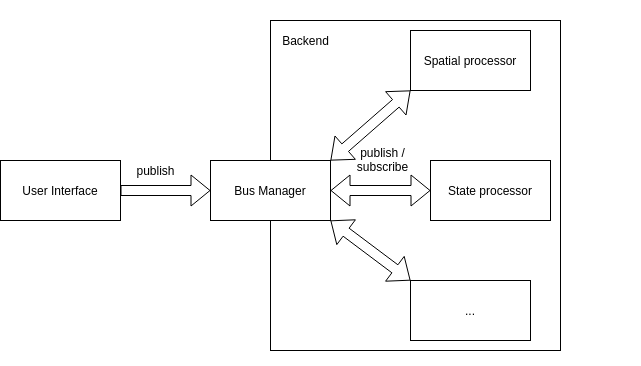
\includegraphics[width=.6\linewidth]{images/couchedit-processors}
  \caption{Publish Subscribe architecture of CouchEdit}
  \label{fig:processors}
\end{figure}

Some of these processors are needed for every type of syntax model, for example the spatial processor, that processes how nodes in the concrete syntax are positioned to each other (above, besides, etc.). Other processors are specific to the given modeling syntax, for example a state chart syntax would require a state processor, that processes if a given graphical object represents a state (usually true if the given node is a rectangle with rounded edges).

A modeling syntax parser for CouchEdit would has to generate these syntax specific processors, while considering multiple design constraints that result from this architecture. Thus a metamodel is needed that can define the desired abstract modeling syntax and specify how a concrete graphical syntax can be mapped to this abstract syntax. While there is ongoing research in the area of relaxed conformance editing and how to link concrete and abstract syntax, it does not immediately become clear what such a metamodel can look like.

\section{Purpose of this Study}
The primary purpose of this study was to develop a metamodel for the CouchEdit framework. This metamodel is supposed to provide a comprehensive and easy to use way for defining new modeling languages. To evaluate the applicability of this metamodel, furthermore a prototypical code generator was implemented, that can comprehend this newly designed metamodel and translate it into a source code implementation.

This extension of the CouchEdit framework is supposed to improve developer accessibility and framework flexibility. While a code generator means that the system still has to be recompiled for every modeling syntax, it still becomes easier to support new modeling syntaxes as the metamodel abstracts away from the actual source code implementation and thus requires less knowledge about the CouchEdit framework.


\section{Thesis Structure}
\dots